%
% boundary.tex -- 
%
% (c) 2019 Prof Dr Andreas Mueller
%
\section{Which boundary points influence a solution in point?
\label{section:which-boundary-points}}
\rhead{Which boundary points influence the solution in a point?}
\begin{figure}
\centering
%\includegraphics{../common/images/kausal-1.pdf}
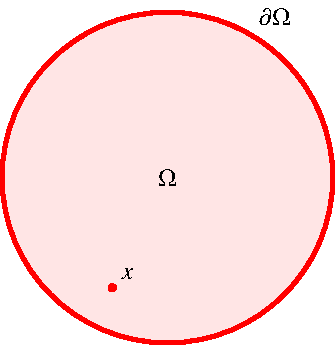
\includegraphics{9-hyperbolic/images/elliptic.pdf}
\qquad\qquad%
%\includegraphics{../common/images/kausal-2.pdf}
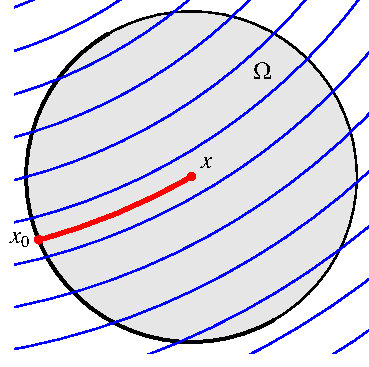
\includegraphics{9-hyperbolic/images/ql.pdf}
\caption{Boundary values of the domain that influence the values of the
solution in a point.
For an elliptic differential equation $\Delta u=f$
(links)
the function values depend on all boundary values and on any value
of the function $f$.
The solution of a quasilinear partial differential equation (right)
in the point $x$ depends on the initial point $x_0$ of a characteristic
through $x$.
\label{einflussmenge1}}
\end{figure}
\begin{figure}
\centering
%\includegraphics{../common/images/kausal-3.pdf}%
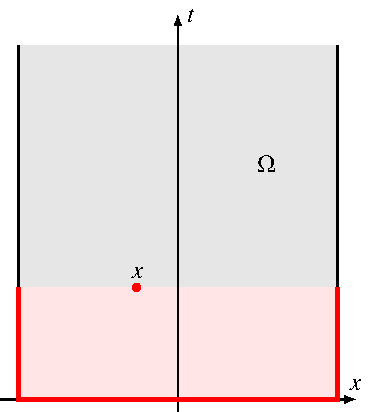
\includegraphics{9-hyperbolic/images/parabolic.pdf}%
\qquad\qquad%
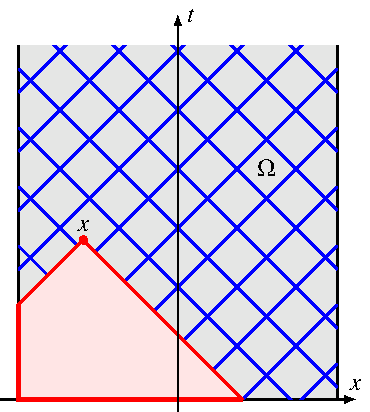
\includegraphics{9-hyperbolic/images/hyperbolic.pdf}%
%\includegraphics{../common/images/kausal-4.pdf}
\caption{Boundary values and points of the domain that influence
the value of a solution.
The solution of a parabolic partial differential equation
at time $t$ depends on all values for times $t'<t$.
For a hypberbolic partial differential equation only the function
values inside a cone emanating back in time from a point $x$ 
influence the value in that point.
\label{einflussmenge2}}
\end{figure}
The theory developed so far allows to give an answer to the question
which points on the boundary or in the interior of the domain have
an influence the solution of the partial differential equation
$Lu=f$.

In chapter~\ref{chapter:elliptic} we have found a formula for the solution
of an elliptic partial differential equation, which computes the 
values in the interior as an function of the values on the boundary
and all values of $f$ in the interior:
\[
u(x)
=
\int_\omega G(x,\xi)f(\xi)\,d\xi
+
\int_{\partial\Omega} \operatorname{grad}_\xi G(x,\xi)g(\xi)\,d\xi.
\]
A change in $g$ anywhere on the boundary or change of $f$ anywhere in the
interior will change the solution everywhere
(figure~\ref{einflussmenge1}, left).

By contrast, in chapter~\ref{chapter:geometry} it was shown that
the value of a solution of quasilinear partial differential
equation of first degree in a point $x$ only depends on the values on
the characteristic that runs through $x$
(figure~\ref{einflussmenge1}, right).

The solution of a parabolic paratial differential equation can also be
expressed using Green's function.
Formula~(\ref{green-parabolisch}) shows, that the values $u(t,x)$
in general depend on all boundary values
$g(t',\xi)$ and internal values $f(t',\xi)$
with $t'<t$ (figure~\ref{einflussmenge2}, left).

The characteristic surfaces (curves) answer this question for hyperbolic
partial differential equations.
The characteristic surfaces (curves) that go through a point $x$
define a cone.
The value of $u(x)$ of the solution in the point $x$ depends on the
function values of the right hand side of the equation and the boundary values
the past cone
(figure~\ref{einflussmenge2}, right).

